\documentclass[
	a4paper, 		%Seitengröße
	11pt,			%Schriftgröße
	DIV=13,			% Satzspiel
%	parskip=none, 	%Maybe unused....
	oneside,
	%twoside,
	cleardoublepage=empty,
	%BCOR=5mm,		%Bindekorrektur
	%openright,		%Chapter fangen immer rechts an
	%draft,
	listof=totoc,		%Tabellen- und Abbildungsverzeichnis im Inhaltsverzeichnis
	%bibliography=totoc,		%Literaturverzeichnis im Inhaltsverzeichnis UNUSED
	toc=flat,
	]{scrreprt}



%Zeilenabstand Faktor 1.63 (Bei 11pt mit Abstand 18pt)
\usepackage{setspace}

%Package um PDF Files zu includieren
\usepackage{pdfpages}

%Erzeugung von Tabellen mit über mehrere Seiten
\usepackage{longtable}

%Absatzabstand
%\usepackage[skip=6pt plus1pt, indent=0pt]{parskip}

%Automatische Verlinkung im Dokument einfügen
\usepackage[
	hidelinks,
	%citecolor=black,
]{hyperref}

%Vorbereitung Mathesymbole
\usepackage{amsmath, amssymb}

%Bildereinbindung
\usepackage{graphicx}
\graphicspath{{bilder/}}
\usepackage{color}

\usepackage{import}

%Tabellen-Pakete
\usepackage{booktabs}

%Literaturverzeichnis
\usepackage{csquotes} %Anführungszeichen

%Erstellung der Kopf- und Fußzeile
\usepackage[
	headsepline, %Trennline
	automark,	
]{scrlayer-scrpage}
\pagestyle{scrheadings}


%\usepackage{blindtext}

% Angaben im Dokument
\title{Projektdokumentation Flugdrohnenprojekt \\
Team Blau}
\author{\textbf{Projektteam:} Alissa Kosin, Christian Schmidt, Daniel Schien, Daniel Stotz,\\ Jan Fischer, Johannes Walz, Kai Wilkowski, Pascal Bornkessel, Tim Gumbold}
\date{Projektdokumentation Flugdrohnenprojekt\\ Studiengang LT \& FFI }
	\publishers{
	\begin{tabular}{rl}
		\textbf{Dozent}	 		& Prof. Dr. A. Soika \\
		\textbf{Dozent} 		& Prof. Dr. L. König \\
		\textbf{Dozent} 		& Prof. Dr. U. Burger \\
		\textbf{Dozent} 		& Prof. Dr. G. Elsbacher \\
		\textbf{Dozent} 		& E. Obermeier \\
		\textbf{Dozent} 		& Prof. Dr. H. Göllinger \\
		\textbf{Abgabedatum}	& 25.06.2023\\
		
	\end{tabular}	
}

\begin{document}
	\titlehead{
		\centering
		\hfil
		
\includegraphics[width=\linewidth]{thi_logo_wb_S}
		\hfil
		
}
	\maketitle
	
	\tableofcontents
	
	%Aenderung des Zeilenabstands auf ca. 18pt
	\setstretch{1.6}
	
	\chapter{Einführung}

In den Studiengängen Flug- und Fahrzeuginformatik (FFI) und Luftfahrttechnik (LT) gibt es im 6ten Studiensemester ein verpflichtendes Projekt. Dieses wird von Projektteams, die aus FFI und LT Studenten besteht, absolviert. Die Inhalte des Projektes werden generisch in den Modulhandbüchern beider Studiengänge beschrieben. Im Modulhandbuch des Studiengangs FFI wird der Inhalt im Entwicklungszyklus des V-Modells beschrieben. Die genannten Schritte sind:
\begin{enumerate}
	\setstretch{1}
	\item Analyse
	\item Recherche zur Lösungsvorbereitung
	\item Beschreibung der Lösung
	\item Auswahl von Methoden und Tools
	\item Implementierung
	\item Verifikation
	\item Erstellung eines Abschlussberichts
	\item Projektbegleitendes Projekt- und Konfigurationsmanagement
\end{enumerate}
\setstretch{1.63}
Im Modulhandbuch des Studiengang LT wird der Inhalt konkreter beschrieben. Das Projekt ist auf dem Gebiet der Luftfahrttechnik und wird als Teamarbeit gelöst. Die wechselnden Randbedingungen der Flugmissionen werden bereits erwähnt. In der verpflichtenden Literatur ist das ausgegebene Lastenheft aufgeführt, welches den zu erbringenden Leistungsumfang definiert.
Das ausgegebene Projekthandbuch konkretisiert das Projektziel mit den Worten: Das Projektziel ist die Erstellung einer senkrecht startenden und landenden Flugdrohne aus verfügbaren und selbst gefertigten Bauelementen sowie der Entwicklung, Fertigung und Integration einer Vorrichtung zur Aufnahme, Beförderung und Absetzen von Lasten. Die Funktion des Systems ist im Rahmen einer vorgegebenen Flugmission nachzuweisen.

\section{Hintergrund des Themas}
Das Ziel der Vorlesung wird ebenfalls in den Modulhandbüchern erläutert. Beide Modulhandbücher legen Wert auf eine selbstständige Teamarbeit um eine Gesamtlösung zu erarbeiten. Es geht um das vollumfängliche Arbeiten in einer Projektumgebung, inklusive des Projektmanagements, der Organisation und der Dokumentation. Die angestrebten Lernergebnisse des Studiengangs LT erwähnen die ingenieurwissenschaftlichen Methoden im besonderen.

Das Projekthandbuch ist im Stile eines Lastenheftes geschrieben. In Kapitel 2 werden allgemeine Definitionen und Rahmenbedingungen beschrieben. Das Projekt wird innerhalb eines Produktentstehungsprozesses (PEP) bearbeitet. Der PEP richtet sich nach dem NASA Systems Engineering Handbook (SP-2016-610S Rev. 2). In diesem Enthalten sind mehrere vorzubereitende Technische Reviews (PDR, CDR, FRR). Im Überblick bleibt zu sagen das in diesem Projekt der Entwicklungszyklus eines Fluggerätes im kleinen Simuliert wird. Das Ziel ist es den Studenten einen Einblick in die Entwicklungsprozesse von luftfahrttechnischen Geräten zu geben. Dazu gehört die abschließende Ausgabe einer THI-Registriernummer und die Erteilung der Permit-to-fly (PTF).

\section{Zusammenfassung} %Problemstellung
Die Aufgabenstellung des Flugprojektes im Sommersemester 2023 (SS23) beinhaltet drei Flugaufgaben (Challenges). Für Challenge \#1 ist eine flugfähige Drohne zu erstellen, die eine definierte Mission autonom abfliegt. Für Challenge \#2 ist eine angebrachte Last mithilfe einer konstruierten Lastaufhängung autonom an einen definierten Ort zu bringen und abzusetzen. Für Challenge \#3 ist die Last maximal oft zu transportieren. Die Einzelnen Challenges werden in späteren Kapiteln weiter beschrieben. Das Team Blau hat hierfür eine Drohne und Lastaufhängung entwickelt. Die Drohne wurde als Quadrocopter ausgelegt und besitzt vier Arme aus Forged Carbon. Die Lastaufhängung ist mithilfe eines Riegels mit Formschluss realisiert, der über einen Servomotor angesteuert wird.
	
	
	\chapter{Studiengruppe}
\label{chap:Studiengruppe}
Das Projektteam besteht aus neun Personen aus den Studiengängen LT und FFI. Einige Teammitglieder bringen durch eine vorherige Ausbildung Fähigkeiten in den Bereichen Herstellung und (Hier weiteres Beispiel einfügen falls möglich) mit. Durch eine abgeschlossene Berufsausbildung zum Mechatroniker (!?) ist Daniel Schien für die Herstellung verantwortlich.
\begin{table}[htb]
	\centering
	\caption{Studiengruppe}
	\label{tab:Studiengruppe_Aemter}
	\begin{tabular}{rl}
		%Sortierung Alphabetisch (Nachname)?
		\textbf{Name} & \textbf{Position}\\
		\toprule
		Pascal Bornkessel & Teammitglied \\
		Jan Fischer & Teamleiter \\
		Tim Gumbold & Konstruktion \\
		Alissa Kosin & Dokumentation \\
		Daniel Schien & Herstellung \\
		Christian Schmidt & Sicherheit \\
		Daniel Stotz & Teammitglied \\
		Johannes Walz & Teammitglied \\
		Kai Wilkowski & Zeitplanung \\
	\end{tabular}
	
\end{table}

\section{Einteilung der Ämter und Arbeitsgruppen}

\section{Organisatorisches}

\subsection{Digital Working Environment}
		
	\chapter{Projektorganisation}
Am ersten Termin des Projektes wurde die Projektaufbauorganisation erstellt und die Verantwortlichkeiten und Befugnisse der Aufgabenträger definiert. Die Organisation folgt dabei der Reinen Projektorganisation, da die Teammitglieder Studenten sind. Eine Linien- oder Matrixorganisation durch die fehlende Unternehmensorganisation nicht gegeben. Durch die Organisation sind die Vorteile der reinen Projektorganisation im Team spürbar gewesen. Die Motivation war hoch, es konnte schnell auf Änderungswünsche reagiert werden und es kam zu keinen nennenswerten Konflikten. In Unternehmen müsste das Projektteam aufgelöst werden. Dieser Nachteil entfällt. 

Die Einteilung der Ämter innerhalb der Studiengruppe ist in \autoref{chap:Studiengruppe} beschrieben. Die Projektablauforganisation folgt dem V-Modell. Die einzelnen Projektabschnitte wurden dabei, wie bereits erwähnt, vom Auftraggeber vorgegeben und die Feinplanung mithilfe eines Projektstrukturplans durchgeführt. In diesem sind die einzelnen Arbeitspakete genannt und zeitlich abgeschätzt worden. Auf dieser Grundlage wurde die Zeitplanung erarbeitet. Anschließend folgte die Beschreibung der Arbeitspakete mit Inputs und Outputs, sowie einer verbesserten zeitlichen Abschätzung. Im folgenden sind die Ergebnisse dieser Planungen beschrieben.
\section{Projektstrukturplan}
\subsection{Zeitplanung}
\subsection{Meilensteintrendanalyse}
\section{Anforderungsliste}
	
	\chapter{Morphologischer Kasten (Ali)}
Als Hilfsmittel zur Konzeptfindung, haben wir uns dazu entschieden einen Morphologischen Kasten für die Drohne und für die Lastaufhängung zu erstellen.
Die Funktion unserer Drohne und der Lastaufhängung werden in Anlehnung an die Anforderungsliste in Teilfunktionen aufgespalten. Zu diesen Teilfunktion werden dann physikalische Wirkprinzipien gefunden und in einer Matrix notiert, dem sogenannten Morphologischen Kasten. Aus diesen Wirkprinzipien entstehen dann Wirkstrukturen, welche dann anhand von technischen und wirtschaftlichen Kriterien bewertet werden. Hier weicht unsere Konzeptionsmethoden vom klassischen Morphologischen Kasten ab, da wir auf eine ausführliche wirtschaftliche Bewertung verzichten. Das Wirkprinzip mit der höchsten relativen Wertung wird dann eventuell mit anderen hochbewerteten Wirkprinzipien ergänzt und bildet dann die Grundlage für unser Gesammtkonzept. 

\section{Drohne}
Wie in Abb \ref{fig:Morphologischer-Kasten-Drohne} gezeigt haben wir unsere Drohne anhand der Anforderungsliste in Teilaufgaben unterteilt und diese verallgemeinert. Für die Aufgaben suchen wir im Team nach Lösungsanzätzen und Wirkprinzipien. Es werden sämtliche Ideen festgehalten ohne vorzeitige Bewertungen.
So wird auch der Vorschlag Holz als mögliches Material aus dem Teile der Drohne hergestellt werden können, wahrgenommen.
% sich für das Material aus dem Teile der Drohne bestehen sollen auch Lösungen wie Holz  

\begin{figure}[h]
	\centering
	\includegraphics[width=1.00\textwidth]
	{bilder/Morphologischer_Kasten/MorphKastDrohne}
	\caption{Morphologischer-Kasten-Drohne}
	%{Beschädigter Stabilisator\cite{Aerossurance}} 
	\label{fig:Morphologischer-Kasten-Drohne}
\end{figure}

Anschließend suchen wir nach Wirkstrukturen. Dabei beachten wir das sich die unterschiedlichen Wirkprinzipien einer Wirkstrucktur auch vertragen. Holz zum Beispiel können wir nicht 3D-Drucken. in der Abbildung sind unsere drei Wirkstrukturen zu sehen.

%\begin{figure}[H]
%	\centering
%	\includegraphics[width= 0.40\textwidth]{Bilder/MorphKastDrohne.jpg}
%	\caption[Beschädigter horizontaler Stabilisator]{Beschädigter Stabilisator %\cite{Aerossurance}} 
%	\label{fig:Morphologischer-Kasten-Drohne}
%\end{figure}


\subsection{Technische Bewertung}
Bei der technischen Bewertung wird den drei Wirkstrukturen eine relative Wertigkeit zugeordnet. Eine wirtschaftliche Bewertung wird hier nicht durchgeführt. Einige wirtschaftliche Aspekte werden trotzdem berücksichtigt. So zum Beispiel das die Materialien weitestgehend an der Thi schon verfügbar sein sollten und nicht nachbestellt werden müssen. Ein weiteres wirtschaftliches Kriterium ist, dass wir unsere Fertigungsteile nach Möglichkeit entweder selbst oder in einer der Werkstätten an der THI fertigen können und dementsprechend keine außerhochschulischen Dienste in Anspruch nehmen müssen.
Weitere Kriterien orientieren sich eher an den Vorstellungen die wir an das Projekt haben. So ist eines unserer Ziele eine möglichst leichte und kompakte Drohne zu entwickeln und trotzdem soll sie robust sein.  Ebenfals ist es uns wichtig möglichst viel selbst herstellen zu können und unsere Arbeit innovativ zu gestalten. Dementsprechend sind die Gewichtungen der Kriterien recht subjektiv. Die Kriterien werden mit eins (unwichtig bzw. vorgegeben) bis vier(sehr wichtig) gewichtet. Jede Wirkstruktur wir unabhängig von den anderen Wirkstrukturen bewertet. Schlißlich werden die Bewertungen aufsummiert und durch die maximal erreichbare Bewertung geteilt sogass sich eine relative Bewertung ergibt. Wie in Abbildung zu sehen hat die 1.Wirkstruktur "Alpha" die höchste relative Wertigkeit und ist somit Grundlage für unser endgültiges Konzept.
\begin{figure}[h!]
	\centering
	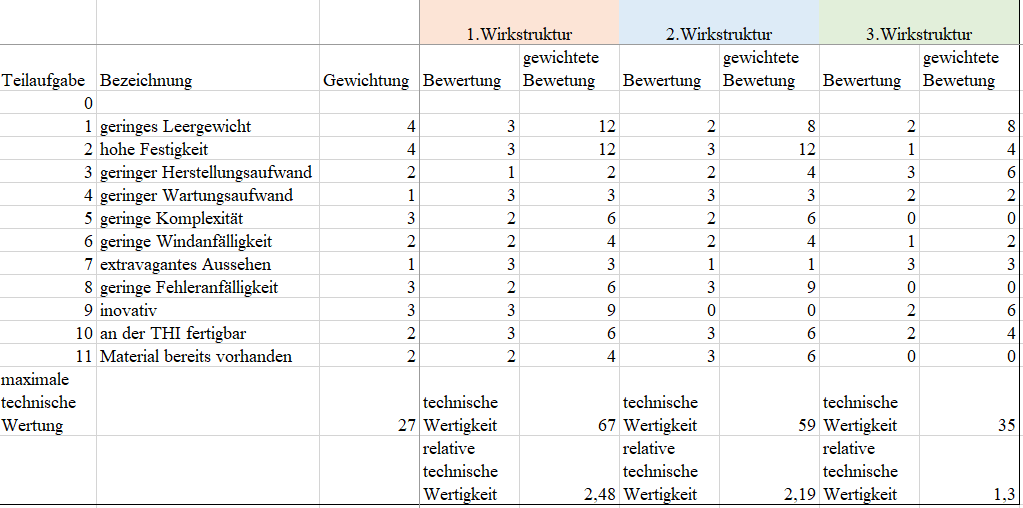
\includegraphics[width= 1.00\textwidth]{bilder/Morphologischer_Kasten/BewDrohne}
	\caption{Technische-Bewertung-Drohne}
	%{Beschädigter Stabilisator\cite{Aerossurance}} 
	%	\label{fig:Morphologischer-Kasten-Drohne}
\end{figure}

\subsection{Stärkendiagramm}



\section{Lastaufhängung}
Für den Morphologischen Kasten der Lastaufhängung wird der gleiche Prozess wie bereits in den Punkten weiter oben beschrieben, angewendet.
Die Überfunktion Lastaufhängung wird in Teilfunktionen aufgeteilt. In Abbildung ist zu erkennen wie für jede Teilaufgabe mindestens drei Lösungselemente gefunden wurden. Im darauffolgenden Schritt werden diese Wirkprinzipien zu Wirkstrukturen verheiratet.
\begin{figure}[h!]
	\centering
	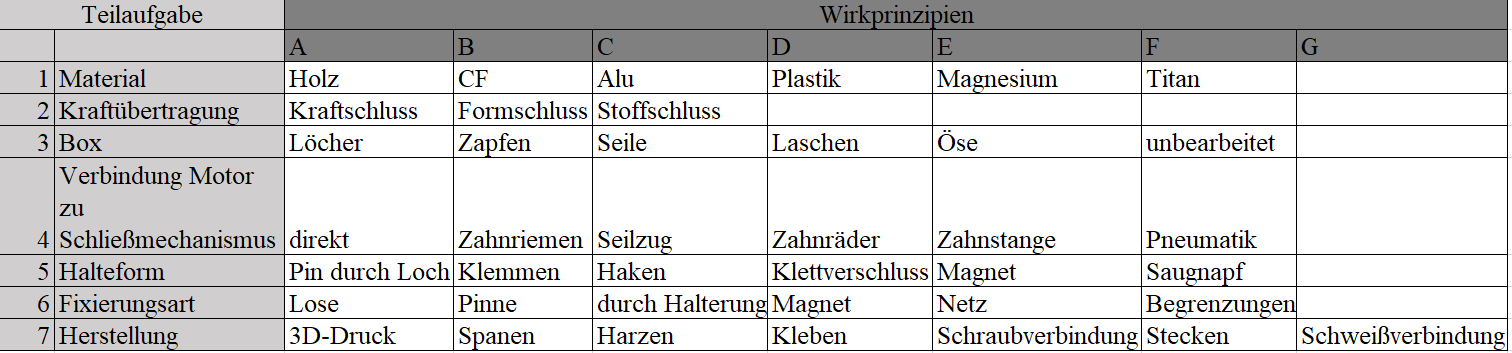
\includegraphics[width= 1.00\textwidth]{bilder/Morphologischer_Kasten/MorphKastLastaufh}
	\caption{Morphologischer-Kasten-Lastaufhaengung}
	%{Beschädigter Stabilisator\cite{Aerossurance}} 
	%	\label{fig:Morphologischer-Kasten-Drohne}
\end{figure}

\subsection{Technische Bewertung}

\begin{figure}[h!]
	\centering
	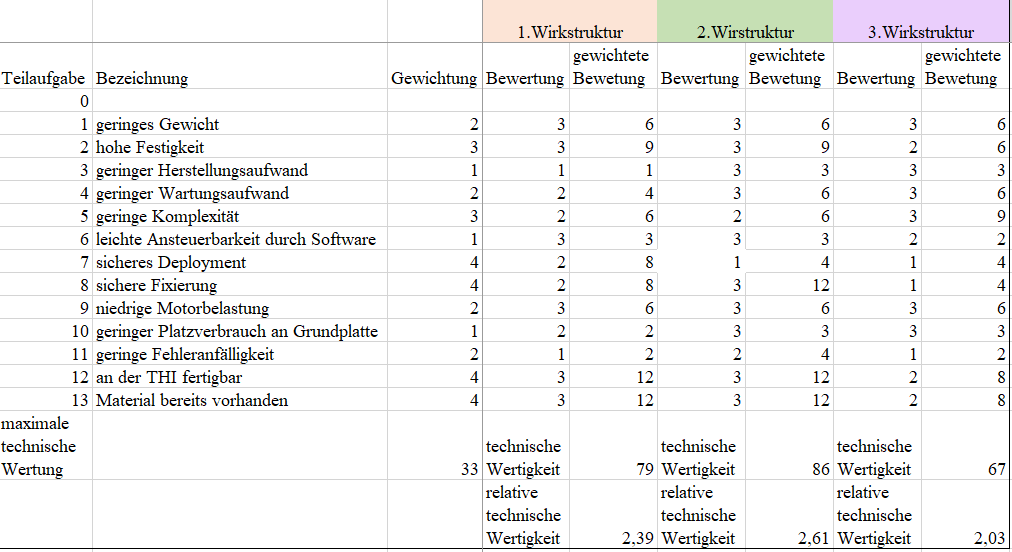
\includegraphics[width= 1.00\textwidth]{bilder/Morphologischer_Kasten/BewLastaufh}
	\caption{Technische-Bewertung-Lastaufhaengung}
	%{Beschädigter Stabilisator\cite{Aerossurance}} 
	%	\label{fig:Morphologischer-Kasten-Drohne}
\end{figure}

\subsection{Stärkendiagramm}


\section{Konzeptauswahl}
	
	\chapter{Entwurf}

\section{Drohne}
\subsection{Werkstoffwahl}
\subsection{Forged Carbon}
\subsection{Skizzen}
\subsection{Sicherheitsanforderungen}


\section{Lastaufhängung}
\subsection{Werkstoffwahl}
\subsection{Skizzen}
\subsection{Sicherheitsanforderungen}


\section{Integration}


	
	\chapter{Berechnung}

\section{Drohne}
\subsection{Ansysberechnung der Ausleger}
\subsection{Flugleistungsberechnung}
\subsection{Schwerpunktanalyse}

\section{Lastaufhängung}

	
	\chapter{Softwareentwicklung}

\section{Drohne}
\subsection{MVP}
\subsection{Funktionsentwicklung}
\subsection{Ansteuerung der Motoren}
\subsection{Q-Ground Control}

\section{Lastaufhängung}
\subsection{Ansteuerung des Servomotors}

	
	\chapter{Kostenplanung}
Eine Anforderung an das Projekt ist die kostengünstige Durchführung. Vom Auftraggeber wurde eine Grundausstattung zur Verfügung gestellt. Das Team Blau hat sich dazu entschieden, dass nach Möglichkeit alle bereitgestellten Bauteile verwendet werden. 
\section{Drohne}
\subsection{Chopped Carbon Tow}


\section{Lastaufhängung}
\subsection{Axiallager}

\section{Gesamtsystem}
	
	\chapter{Ausarbeitung}

\section{Erzeugnisgliederung}
\subsection{Fertigungszeichnungen}
\subsection{Stückliste}


\section{Herstellung}
\subsection{Materialbeschaffung}
\subsection{Forged Carbon Ausleger}
\subsection{Erstellung Ersatzausleger}
\subsection{Montageanleitung}
\subsection{Montage}



	
	\chapter{Test Bench}

\section{Drohne}

\section{Lastaufhängung}
\subsection{Prototyp Herstellung}
\subsection{Testdurchführung}
\subsection{Testergebnisse}
\subsection{Optimierungen}

\section{1.Freiflugtag}
\section{2.Freiflugtag}

	
	\chapter{Abschluss}

\section{Konzeptfreigabe}

\section{Baufreigabe}

\section{Flugfreigabe}

	\listoffigures
	
	\listoftables
	
\end{document}